\documentclass[a4paper,12pt]{article}

% Packages
\usepackage{amsmath} % For mathematical symbols and formulas
\usepackage{geometry} % For adjusting the page layout
\usepackage{enumitem} % For better control over lists
\usepackage{hyperref}
\usepackage{parskip}
\usepackage{graphicx}
\setlength{\parindent}{0pt}

% Page layout settings
\geometry{left=2.cm, right=2.cm, top=2.cm, bottom=2.4cm}

\title{\vspace{-1cm}\Huge{ASTR4004/ASTR8004 2026\\Astronomical Computing Assignment 3}}
\author{Sven Buder}
\date{\textbf{due Thursday, 3 September, 2026}}

\begin{document}

\maketitle

This assignment is worth \textbf{20 points}. All necessary files can be found at \url{https://github.com/svenbuder/astro_comp_assignment02_2026} and its \texttt{data/} directory.
Complete the analysis in Jupyter notebooks and upload all code/notebooks and figures to your GitHub repository. Add Markdown cells for short explanations and answers.
Tasks with a $\star$ require more independent choices or interpretation and are intended to distinguish strong submissions.
Figures should be clearly labelled and suitable for communicating your results to another astronomer.

\section{\texttt{git} in Practice \hfill [2 points]}

Being able to share code and collaborate on projects is essential in both astronomical research and data science. Use a GitHub repository to track your work throughout this assignment.
Demonstrate that you can:

\begin{itemize}
    \item initialise a repository and push content to the \textit{main} branch;
    \item create and work on a branch with a descriptive name;
    \item make regular commits with meaningful commit messages;
    \item merge your branch back into \textit{main}.
\end{itemize}

Maintain a clear directory structure, with data in \texttt{data/} and figures in \texttt{figures/}.

Submit the link to your GitHub repository and specify your main working branch if it differs from \textit{main}.

\section{Bright Stars Around M67 with ADQL \hfill [6 points]}

A colleague is interested in the open cluster Messier 67 (RA = 132.825 deg, Dec = 11.8 deg) and is considering an observation proposal using the 2dF fibre positioner and HERMES spectrograph (effective for Gaia G band magnitudes $<$ 14) to follow up stars observed with the APOGEE spectrograph (for which they only have 2MASS catalogue identifiers). They need to know if there are enough bright stars in this region for observation. Your task is to assist by querying data from Gaia DR3 and performing some basic analysis.

\begin{enumerate}

    \item Write an ADQL query that returns all stars stars in Gaia DR3 (\texttt{gaiadr3.gaia\_source}) table) within $1$ degree of M67 with $G<14$ (\texttt{phot\_g\_mean\_mag}) and crossmatches them with 2MASS (\texttt{gaiadr1.tmass\_original\_valid}). Include your ADQL query in the notebook and report the number of returned stars.

    \item Identify stars with:
    \begin{itemize}
        \item bad 2MASS photometry (\texttt{ph\_qual} is not \texttt{'AAA'});
        \item non-positive Gaia \texttt{parallax}es.
    \end{itemize}
    Apply these quality cuts and report how many stars remain.

    \item Create a two-panel figure showing:
    \begin{itemize}
        \item Gaia BP$-$RP versus absolute $G$ magnitude, using \texttt{bp\_rp};
        \item 2MASS J$-$Ks versus apparent $H$ magnitude, using \texttt{j\_m}, \texttt{h\_m}, and \texttt{ks\_m}.
    \end{itemize}

    Save the figure as \texttt{figures/cmds\_M67.png}.

    \item $\star$ Based only on fibre usage, would you recommend this field for a 2dF/HERMES observing proposal? Support your answer quantitatively.

\end{enumerate}

\section{Radial Metallicity Relations in Simulations \hfill [6 pts]}

The radial metallicity relation is a function that describes the change of metallicity - here the gas phase metallicity $\mathrm{A(O)} = \log_{10}(N_\mathrm{O}/N_\mathrm{H}) + 12$ - along the galactocentric cylindrical radius $R_\mathrm{Gal.}$. Understanding the radial metallicity gradient in galaxies provides critical insights into their formation and evolutionary processes, such as inside-out formation, gas accretion, outflows, and radial migration. A lot of work has been done through observational studies (e.g. Ho et al., 2017, ApJ, 846, 39) and a few simulations (e.g. Grand et al., 2016, MNRAS, 460, 94), but more works needs to be done to understand the radial metallicity gradient!

Your colleague has just finished an exciting cosmological simulation that traces the gas phase metallicity for a Milky Way analogue, that is, a spiral galaxy. They have limited the simulation data to the positions (x, y, z) of the innermost gas particles ($R_\mathrm{Gal.} < 25\,\mathrm{kpc}$) and their gas phase metallicity $\mathrm{A(O)}$ and uploaded them as a FITS file for you at:

\texttt{data/nihao\_uhd\_simulation\_g8.26e11\_xyz\_positions\_and\_oxygen\_ao.fits}.

\subsection{Task}

Download the file from the link above into \texttt{data/}. Load the file with \texttt{python} and then perform the following tasks to create figures that are saved in \texttt{figures/}:

\begin{itemize}
\item Plot a 2-panel figure:
    \begin{itemize}
    \item (a) Logarithmic density plot of $R_\mathrm{Gal.}$ vs. $\mathrm{A(O)}$, with a linear fit and legend.
    \item (b) Residuals of the fit, $R_\mathrm{Gal.}$ vs. $\Delta \mathrm{A(O)}$.
    \end{itemize}
\item Use a \texttt{python} fitting tool to fit a linear function to the data, reporting the intercept and slope with uncertainties. Include any hyperparameters used.
\item  $\star$ Discuss where the linear model fits well and where it does not. Use statistical metrics, such as the root mean squares or other goodness-of-fit indicators, to quantify the performance of your linear fit in general and regions with larger residuals.
\item Plot a 3-panel figure for the $x$ vs. $y$ plane using the same bins and sensible colormaps:
    \begin{itemize}
    \item (a) 2D-histogram of the median simulated $\mathrm{A(O)}$.
    \item (b) 2D-histogram of the median fitted $\mathrm{A(O)}$
    \item (c) 2D-histogram of the median residuals $\Delta \mathrm{A(O)}$.
    \end{itemize}
\item Describe your choice of 2D bins. Discuss what details would be missed with fewer bins or problems encountered with more bins.
\item $\star$ Analyze the residuals in more detail and propose an explanation for any patterns you observe.
\end{itemize}

\section{Stellar spectrum reduction \hfill [6 points]}

Veloce is a high-resolution echelle spectrograph. The supplied files
\texttt{data/flat.fits} and \texttt{data/moon.fits} contain the same
$4112\times385$ pixel region of the detector around the Ca\,II triplet
($\sim851$--$871\,\mathrm{nm}$). The figure below shows these data. 

\vspace{-0.5cm}
\begin{figure}[h!]
    \centering
    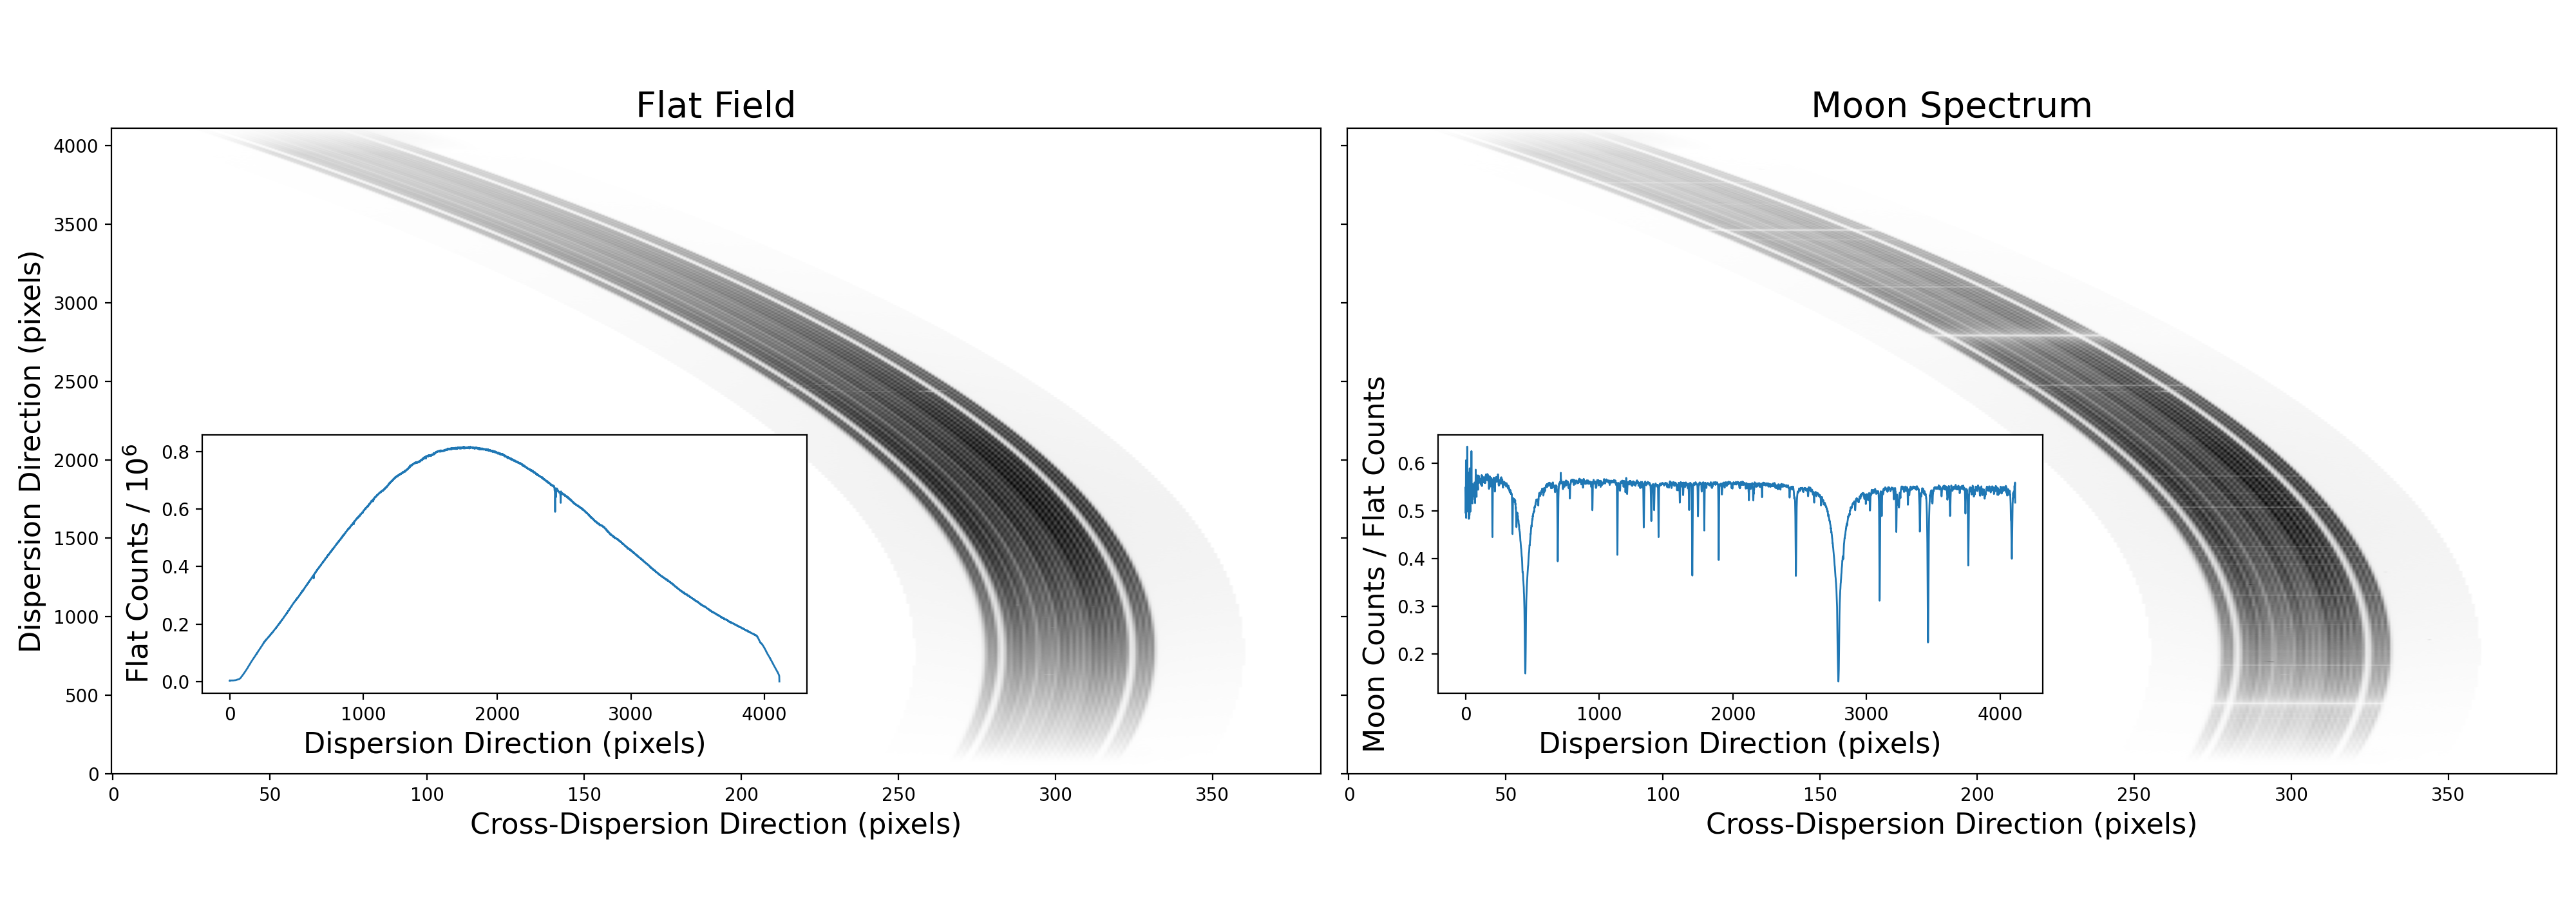
\includegraphics[width=\textwidth]{figures/veloce_flat_moon_cutouts.png}
    \caption{Cut-outs of a Veloce flat-field exposure (left) and Moon exposure (right). The inset panels illustrate simple sums across the cross-dispersion direction.}
    \label{fig:veloce_cutouts}
\end{figure}


The dispersion direction runs vertically and the cross-dispersion direction horizontally. The central group of traces contains the science fibres, with sky fibres on either side separated by less illuminated gaps. The curved boundaries following the science fibres are referred to here as the \textit{tramlines}.
For this simplified exercise, all neighbouring tramlines have been removed and you may assume that the separation between the left and right tramline edges in the cross-dispersion direction is constant.

\begin{enumerate}

    \item $\star$ Use the flat-field image to determine the location of the science fibres as a function of dispersion pixel. Fit an appropriate smooth function to describe the curvature of the order and briefly explain your approach. In case you do not succeed before the deadline, you can simply sum across \texttt{axis=1}.

    \item Plot the flat-field image with your fitted tramlines overlaid to demonstrate that they follow the science fibres across the detector.

    \item Use the same tramlines to extract both the flat-field and Moon spectra by summing the counts in the cross-dispersion direction. Divide the extracted Moon spectrum by the extracted flat-field spectrum and plot the result as a function of dispersion pixel and indicate the pixels of the three strong Ca II lines 8498, 8542 and $8662\,\mathrm{\AA}$.

\end{enumerate}

A successful solution does not require a particular fitting method or polynomial order. The goal is to develop and test a \textit{reasonable} method that works for these data.


\end{document}